\documentclass[svgnames]{beamer}
\mode<presentation>
\usefonttheme{serif}
\usecolortheme{dove}
\useinnertheme{rounded}
%\useoutertheme{smoothbars}
\setbeamercolor{item projected}{fg=black}
\setbeamertemplate{navigation symbols}{}

\usepackage[english]{babel}
\usepackage[latin1]{inputenc}
\usepackage{times}
\usepackage{amsthm,amssymb,amsmath,graphicx}
\usepackage{color}
\usepackage{gastex}
\usepackage{framed}
\usepackage{graphicx}
\usepackage{multicol}
\usepackage{ulem}
\usepackage{ifthen}
\usepackage{tikz}

%%%%%%%%%%%%%%%%%%%%%%%%%%%%%%%%%%%%%%%%%%%%%%%%%%%%%%%%%%%%%%%%%%%%%%%%%%%%%%%%%%%%%%%%
%%%%%%%%%%%%%%%%%%%% A non-original creation by Nathanaël Fijalkow and Victor Marsault %

\setbeamertemplate{frametitle}{
  \vskip-2pt
  \begin{beamercolorbox}[rightskip=2cm,leftskip=1em,dp=1ex,wd=12.8cm]{frametitle}
    \vskip2pt
    \usebeamercolor{frametitle}
    \begin{tikzpicture}
      \useasboundingbox (0,0) rectangle (0,0); 
      \ifthenelse{\insertframenumber<\inserttotalframenumber}
      { 
        \pgfmathsetmacro{\aimangle}{90-(\insertframenumber*360/\inserttotalframenumber)}
        \fill [fill=frametitle.fg,thin, color=gray!50,draw=black] (11.8,.2) -- (11.8,.6) arc (90:\aimangle:0.4) -- cycle;

      }{ 
        \fill[fill=frametitle.fg,thin, color=gray!50,draw=black] (11.8,0.2) circle (.4);
      }
      \fill[fill=frametitle.fg,thin, color=white,draw=black] (11.8,0.2) circle (.3);
      \node at (11.8, .2) [black,circle]{\normalsize\insertframenumber};
    \end{tikzpicture}
    \insertframetitle
    \vskip2pt
  \end{beamercolorbox}
}
%%%%%%%%%%%%%%%%%%%%%%%%%%%%%%%%%%%%%%%%%%%%%%%%%%%%%%%%%%%%%%%%%%%%%%%%%%%%%%%%%%%%%%%

\setbeamertemplate{blocks}[rounded]
\setbeamercolor{block title}{bg=normal text.bg!90!black}
\setbeamercolor{block body}{bg=normal text.bg!95!black}

\renewcommand{\AA}{\mathcal{A}}

\newcommand{\PSPACE}{\mathrm{PSPACE}}
\newcommand{\BB}{\mathcal{B}}
\newcommand{\CC}{\mathcal{C}}
\newcommand{\JJ}{\mathcal{J}}
\newcommand{\DD}{\mathcal{D}}
\newcommand{\KK}{\mathcal{K}}
\newcommand{\LL}{\mathcal{L}}
\newcommand{\HH}{\mathcal{H}}
\newcommand{\GG}{\mathcal{G}}
\newcommand{\RR}{\mathbb{R}}
\newcommand{\NN}{\mathbb{N}}
\newcommand{\QQ}{\mathbb{Q}}
\newcommand{\MM}{\mathcal{M}}
\newcommand{\MMAA}{\MM_\AA}
\newcommand{\tr}[1]{\langle #1 \rangle}
\newcommand{\prob}[1]{\mathbb{P}_{#1}}
\newcommand{\stab}[1]{S(#1)}
\newcommand{\set}[1]{\{ #1 \}}
\newcommand{\val}[1]{\text{val}(#1)}

\newcommand{\ProA}{\widehat{A^*}}
\newcommand{\ProProA}{\widetilde{A^*}}
\newcommand{\PPA}[1]{\ProProA[#1]}

\renewcommand{\P}{\mathbb{P}}

\newtheorem{conjecture}{Conjecture}
  
\title{The Value $1$ Problem\\
for Probabilistic Automata}
\subtitle{Bruxelles}
\author{Nathana\"el Fijalkow}
\institute{LIAFA, Universit\'e Denis Diderot - Paris 7, France\\
Institute of Informatics, Warsaw University, Poland\\
\textbf{nath@liafa.univ-paris-diderot.fr}}

\date{June 20th, 2014}

\AtBeginSection[]
{
\addtocounter{framenumber}{-1}
  \begin{frame}<beamer>{Outline}
    \tableofcontents[currentsection]
  \end{frame}
}

\AtBeginSubsection[]
{
\addtocounter{framenumber}{-1}
  \begin{frame}<beamer>{Outline}
    \tableofcontents[currentsection,currentsubsection]
  \end{frame}
}

\begin{document}

\addtocounter{framenumber}{-1}

\begin{frame}
  \titlepage
\end{frame}

\begin{frame}{Probabilistic automata (Rabin, 1963)}
\begin{figure}
\begin{center}
\begin{picture}(20,40)(0,-10)
	\gasset{Nw=6,Nh=6}

  	\node[Nmarks=i,iangle=0](L1)(15,15){$1$}
  	\node(L2)(0,30){$2$}
  	\node[Nmarks=r](L3)(0,0){$3$}

  	\drawedge(L1,L2){$b$}
  	\drawedge[curvedepth=-5,ELside=r](L1,L3){$a,0.4$}
  	\drawedge[curvedepth=-5,ELside=r](L3,L1){$b$}
	\drawloop(L1){$a,0.6$}
	\drawloop[loopangle=135](L2){$a,b$}
	\drawloop[loopangle=215](L3){$a$}
\end{picture}
\end{center}
\end{figure}
$$\prob{\AA} : A^* \rightarrow [0,1]$$
$$\prob{\AA}(w) \textrm{ is the probability that a run for } w \textrm{ ends up in } F$$
\end{frame}

\begin{frame}{The value $1$ problem}
\begin{center}
This talk is about the value $1$ problem:
\end{center}
\begin{framed}
INPUT: $\AA$ a probabilistic automaton\\
OUTPUT: for all $\varepsilon > 0$, there exists $w \in A^*$,
$\prob{\AA}(w) \ge 1 - \varepsilon$.
\end{framed}
\vskip1em
In other words, define $\val{\AA} = \sup_{w \in A^*} \prob{\AA}(w)$, is $\val{\AA} = 1$?
\pause
\vskip1em
It is undecidable (Gimbert and Oualhadj, 2010).

\begin{center}
\begin{huge}
But \textit{to what extent}?
\end{huge}
\end{center}
\end{frame}

\begin{frame}{Objective}
\begin{center}
Construct an algorithm to decide the value $1$ problem,\\
which is \textit{often} correct.
\vskip2em
\pause
Quantify \textit{how often}.
\vskip2em
\pause
Argue that you cannot do \textit{more often} than that.
\end{center}
\end{frame}

\addtocounter{framenumber}{-1}
\begin{frame}<beamer>{Outline}
\tableofcontents
\end{frame}

\section{Theory}

\subsection{A first attempt: get rid of numerical values}

\begin{frame}{At first thought}
\begin{center}
\begin{huge}
Does the \textit{undecidability} come from the \textit{numerical} values?
\end{huge}
\end{center}
\pause
Consider \textit{numberless} probabilistic automata:
\begin{figure}
\begin{center}
\begin{picture}(20,15)(0,5)
	\gasset{Nw=6,Nh=6}

  	\node[Nmarks=i,iangle=180](1)(0,5){$1$}
  	\node[Nmarks=r](2)(20,5){$2$}

	\drawloop(1){$a$}
  	\drawedge(1,2){$a$}
	\drawloop(2){$a$}
\end{picture}
\end{center}
\end{figure}

Two decision problems:
\begin{itemize}
	\item for all $\Delta$, $\textrm{val}(\AA[\Delta]) = 1$,
	\item there exists $\Delta$, such that $\textrm{val}(\AA[\Delta]) = 1$.
\end{itemize}
\end{frame}

\begin{frame}{No future (in this direction)}

\begin{theorem}[F., Horn, Gimbert and Oualhadj]
There is no algorithm such that:

On input $\AA$ (a non-deterministic automaton),
\begin{itemize}
	\item if for all $\Delta$, $\textrm{val}(\AA[\Delta]) = 1$ then ``YES'',
	\item if for all $\Delta$, $\textrm{val}(\AA[\Delta]) < 1$ then ``NO'',
	\item anything in the other cases.
\end{itemize}
\end{theorem}
\end{frame}

\subsection{A second attempt: the Markov Monoid Algorithm}

\begin{frame}{An example}
\begin{figure}
\begin{center}
\begin{picture}(60,15)(0,-5)
	\gasset{Nw=6,Nh=6,loopdiam=6}

  	\node[Nmarks=i,iangle=-90](0)(20,5){$0$}
  	\node(1)(40,5){$1$}
  	\node[Nmarks=r](F)(60,5){$F$}
  	\node(bottom)(0,5){$\perp$}

	\drawloop(0){$a$}
	\drawloop(1){$a$}
	\drawloop[loopangle=0](F){$a,b$}
	\drawloop[loopangle=180](bottom){$a,b$}

  	\drawedge(0,bottom){$b$}
  	\drawedge[curvedepth=2](0,1){$a$}
  	\drawedge[curvedepth=2](1,0){$b$}
  	\drawedge(1,F){$b$}
\end{picture}
\invisible<1,5,6>{
\begin{picture}(60,10)(0,0)
	\gasset{Nw=5,Nh=5,loopdiam=4}

	\put(-20,4){$\tr{a}$}

  	\node(0)(20,5){$0$}
  	\node(1)(40,5){$1$}
  	\node[Nmarks=r](F)(60,5){$F$}
  	\node(bottom)(0,5){$\perp$}

	\drawloop(0){}
	\drawloop(1){}
	\drawloop[loopangle=0](F){}
	\drawloop[loopangle=180](bottom){}

  	\drawedge(0,1){}
\end{picture}}
\invisible<1,2,4,6>{
\begin{picture}(60,10)(0,0)
	\gasset{Nw=5,Nh=5,loopdiam=4}

	\put(-20,4){$\tr{b}$}

  	\node(0)(20,5){$0$}
  	\node(1)(40,5){$1$}
  	\node[Nmarks=r](F)(60,5){$F$}
  	\node(bottom)(0,5){$\perp$}

	\drawloop[loopangle=0](F){}
	\drawloop[loopangle=180](bottom){}

  	\drawedge(0,bottom){}
  	\drawedge(1,0){}
  	\drawedge(1,F){}
\end{picture}}
\invisible<1,2,3,6>{
\begin{picture}(60,10)(0,0)
	\gasset{Nw=5,Nh=5,loopdiam=4}

	\put(-20,4){$\tr{a^\sharp}$}

  	\node(0)(20,5){$0$}
  	\node(1)(40,5){$1$}
  	\node[Nmarks=r](F)(60,5){$F$}
  	\node(bottom)(0,5){$\perp$}

	\drawloop(1){}
	\drawloop[loopangle=0](F){}
	\drawloop[loopangle=180](bottom){}

  	\drawedge(0,1){}
\end{picture}}
\invisible<1,2,3,4>{
\begin{picture}(60,10)(0,0)
	\gasset{Nw=5,Nh=5,loopdiam=4}

	\put(-22,4){$\tr{a^\sharp \cdot b}$}

  	\node(0)(20,5){$0$}
  	\node(1)(40,5){$1$}
  	\node[Nmarks=r](F)(60,5){$F$}
  	\node(bottom)(0,5){$\perp$}

	\drawloop(0){}
	\drawloop[loopangle=0](F){}
	\drawloop[loopangle=180](bottom){}

  	\drawedge[curvedepth=-4](0,F){}
  	\drawedge(1,0){}
  	\drawedge(1,F){}
\end{picture}}
\invisible<1,2,3,4,5>{
\begin{picture}(60,10)(0,0)
	\gasset{Nw=5,Nh=5,loopdiam=4}

	\put(-25,4){$\tr{(a^\sharp \cdot b)^\sharp}$}

  	\node(0)(20,5){$0$}
  	\node(1)(40,5){$1$}
  	\node[Nmarks=r](F)(60,5){$F$}
  	\node(bottom)(0,5){$\perp$}

	\drawloop[loopangle=0](F){}
	\drawloop[loopangle=180](bottom){}

  	\drawedge[curvedepth=-4](0,F){}
  	\drawedge(1,F){}
\end{picture}}
\end{center}
\end{figure}
\pause\pause\pause\pause\pause\pause
\end{frame}

\begin{frame}{Stabilization monoids (Colcombet)}
This is an algebraic structure with two operations:
\begin{itemize}
	\item binary composition
	\item stabilization, denoted $\sharp$.
\end{itemize}
\end{frame}

\begin{frame}{Boolean matrices representations}
\vspace*{1em}
\begin{figure}
\begin{center}
\begin{picture}(60,14)(0,0)
	\gasset{Nw=6,Nh=6,loopdiam=6}

  	\node[Nmarks=i,iangle=-90](0)(20,5){$0$}
  	\node(1)(40,5){$1$}
  	\node[Nmarks=r](F)(60,5){$F$}
  	\node(bottom)(0,5){$\perp$}

	\drawloop(0){$a$}
	\drawloop(1){$a$}
	\drawloop[loopangle=0](F){$a,b$}
	\drawloop[loopangle=180](bottom){$a,b$}

  	\drawedge(0,bottom){$b$}
  	\drawedge[curvedepth=2](0,1){$a$}
  	\drawedge[curvedepth=2](1,0){$b$}
  	\drawedge(1,F){$b$}
\end{picture}
\end{center}
\end{figure}
\vspace*{1em}

$$\tr{a} = 
\left(\begin{array}{cccc}
1 & 0 & 0 & 0 \\
0 & 1 & 1 & 0 \\
0 & 0 & 1 & 0 \\
0 & 0 & 0 & 1
\end{array}\right)
\qquad
\tr{b} = 
\left(\begin{array}{cccc}
1 & 0 & 0 & 0 \\
1 & 0 & 0 & 0 \\
0 & 1 & 1 & 0 \\
0 & 0 & 0 & 1
\end{array}\right)$$

\vspace*{1em}

$$I \cdot \tr{u} \cdot F = 1 \quad \textrm{ if and only if } \quad \prob{\AA}(u) > 0$$
\end{frame}

\begin{frame}{Defining stabilization}
\vspace*{3em}
\begin{figure}
\begin{center}
\begin{picture}(20,10)(0,0)
	\gasset{Nw=6,Nh=6}

  	\node[Nmarks=i,iangle=180](1)(0,5){$1$}
  	\node[Nmarks=r](2)(20,5){$2$}

	\drawloop(1){$a$}
  	\drawedge(1,2){$a$}
	\drawloop(2){$a$}
\end{picture}
\end{center}
\end{figure}
\vspace*{1.5em}
$$\only<1,2,3>{
\tr{a} = 
\left(\begin{array}{ccc}
1 & 1 \\
0 & 1
\end{array}\right)
	}
\qquad
\only<2,3>{
\tr{a^\sharp} = 
\left(\begin{array}{ccc}
0 & 1\\
0 & 1
\end{array}\right)}$$
\vspace*{1em}
In $\tr{a}$, the state $1$ is transient and the state $2$ is recurrent.

\vspace*{1em}
$$\only<3>{M^\sharp(s,t) = 
\left\{\begin{array}{ll}
1 & \textrm{if } M(s,t) = 1 \textrm{ and } t \textrm{ recurrent in } M,\\
0 & \textrm{otherwise.}
\end{array}\right.}$$
\vspace*{10em}
\end{frame}


\begin{frame}{The Markov Monoid Algorithm}
Compute a monoid inside the \textbf{finite} monoid $\MM_{Q \times Q}(\set{0,1},\vee,\wedge)$.

\begin{itemize}
	\item Compute $\tr{a}$ for $a \in A$:
$$\tr{a}(s,t) = 
\left\{\begin{array}{ll}
1 & \textrm{if } \prob{\AA}(s \xrightarrow{a} t) > 0,\\
0 & \textrm{otherwise.}
\end{array}\right.$$	
	\item Close under product and stabilization.
	\item \pause If there exists a matrix $M$ such that 
	$$\forall t \in Q, \quad M(s_0,t) = 1 \Rightarrow t \in F$$
	then ``$\AA$ has value $1$'',
	otherwise ``$\AA$ does not have value $1$''.
\end{itemize}
\end{frame}

\begin{frame}{Correctness}
\begin{theorem}
If there exists a matrix $M$ such that 
$$\forall t \in Q, \quad M(s_0,t) = 1 \Rightarrow t \in F$$
then $\AA$ has value $1$.
\end{theorem}
\pause
But the value $1$ problem is undecidable, so\ldots
\end{frame}

\begin{frame}{No completeness}
\begin{figure}
\begin{center}
\begin{picture}(60,35)(0,0)
	\gasset{Nw=7,Nh=7}

  	\node[Nmarks=i,iangle=-90](0)(30,15){$0$}
  	\node(L1)(0,10){$L_1$}
  	\node[Nmarks=r](L2)(0,30){$L_2$}
  	\node(R1)(60,10){$R_1$}
  	\node(R2)(60,30){$R_2$}

	\drawloop(0){$a$}

  	\drawedge[curvedepth=5,ELside=l](0,L1){$b,\frac{1}{2}$}
  	\drawedge[curvedepth=5,ELside=l](L1,0){$a,1-x$}
  	\drawedge(L1,L2){$b$}
	\drawloop[loopangle=-135](L1){$a,x$}
	\drawloop[loopangle=90](L2){$a,b$}

  	\drawedge[curvedepth=-5,ELside=r](0,R1){$b,\frac{1}{2}$}
  	\drawedge[curvedepth=-5,ELside=r](R1,0){$a,x$}
  	\drawedge[ELside=r](R1,R2){$b$}
	\drawloop[loopangle=-45](R1){$a,1-x$}
	\drawloop(R2){$a,b$}
\end{picture}
\end{center}
\end{figure}

Left and right parts are symmetric, so for all $M$:
$$M(0,L_2) = 1 \Longleftrightarrow M(0,R_2) = 1.$$

Yet: it has value $1$ if and only if $x > \frac{1}{2}$.
\end{frame}

\begin{frame}{A leak}
\begin{figure}
\begin{center}
\begin{picture}(50,30)(0,0)
	\gasset{Nw=6,Nh=6}

  	\node[Nmarks=i,iangle=0](L1)(15,15){$1$}
  	\node(L2)(0,30){$2$}
  	\node[Nmarks=r](L3)(0,0){$3$}

  	\drawedge(L1,L2){$b$}
  	\drawedge[curvedepth=-5,ELside=r](L1,L3){$a$}
  	\drawedge[curvedepth=-5,ELside=r](L3,L1){$b$}
	\drawloop(L1){$a$}
	\drawloop[loopangle=135](L2){$a,b$}
	\drawloop[loopangle=215](L3){$a$}

	\drawline[linewidth=.3,AHnb=0](26,-3)(26,40)

\pause

	\put(45,-10){$\tr{a^\sharp \cdot b}$}

  	\node(L1b)(55,15){$1$}
  	\node(L2b)(40,30){$2$}
  	\node[Nmarks=r](L3b)(40,0){$3$}

  	\drawedge(L3b,L1b){}
	\drawloop(L1b){}
	\drawloop[loopangle=135](L2b){}

\only<3>{\drawedge[dash={1}0](L1b,L2b){$\varepsilon$}}
\end{picture}
\end{center}
\end{figure}
\pause
\vskip2em
\begin{center}
There is a leak from $1$ to $2$.
\end{center}
\pause
\begin{definition}
An automaton $\AA$ is leaktight if it has no leak.
\end{definition}
\end{frame}

\begin{frame}{Leaktight automata}
\begin{theorem}[F.,Gimbert and Oualhadj 2012]
The algorithm is complete for leaktight automata.

Hence, the value $1$ problem is decidable for leaktight automata.
\end{theorem}

\vskip2em
The proof relies on Simon's factorization forest theorem.
\end{frame}

\begin{frame}{Other decidable subclasses: in 2012}
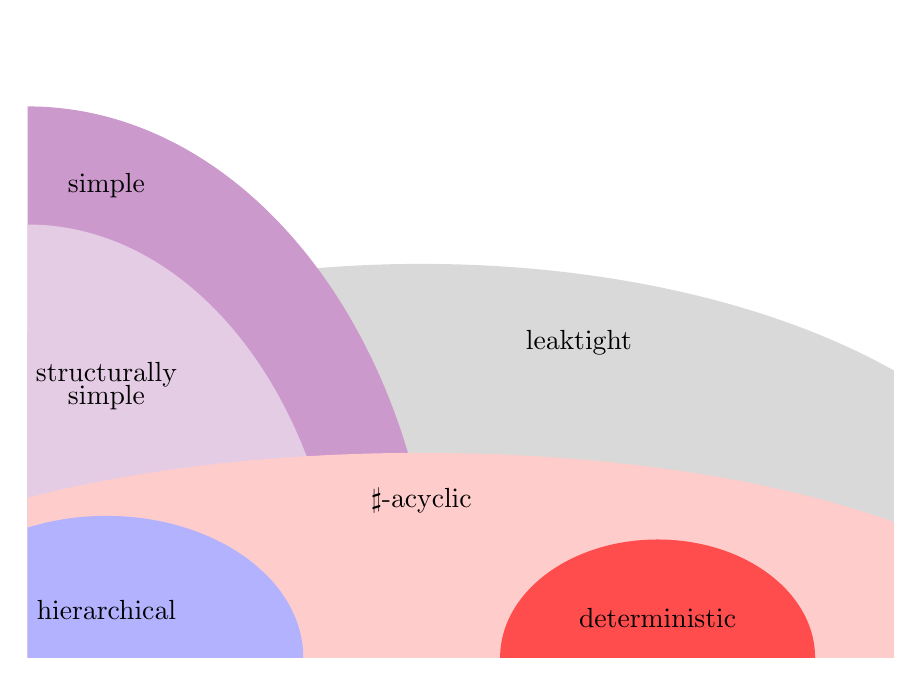
\begin{tikzpicture}
\clip (-6,0) rectangle (5,8);

\fill[white!85!black] (-1,1) ellipse (8cm and 4cm) ;
\draw (1,4) node {leaktight} ;

\fill[white!60!violet] (-6,0) ellipse (5.2cm and 7cm) ;
\draw (-5,6) node {simple} ;

\fill[white!80!violet] (-6,0) ellipse (4cm and 5.5cm) ;
\draw (-5,3.6) node {structurally} ;
\draw (-5,3.3) node {simple} ;

\fill[white!80!red] (-1,0) ellipse (8cm and 2.6cm) ;
\draw (-1,2) node {$\sharp$-acyclic} ;

\fill[white!70!blue] (-5,0) ellipse (2.5cm and 1.8cm) ;
\draw (-5,.6) node {hierarchical} ;

\fill[white!30!red] (2,0) ellipse (2cm and 1.5cm) ;
\draw (2,.5) node {deterministic} ;
\end{tikzpicture}
\end{frame}

\begin{frame}{Other decidable subclasses: today}
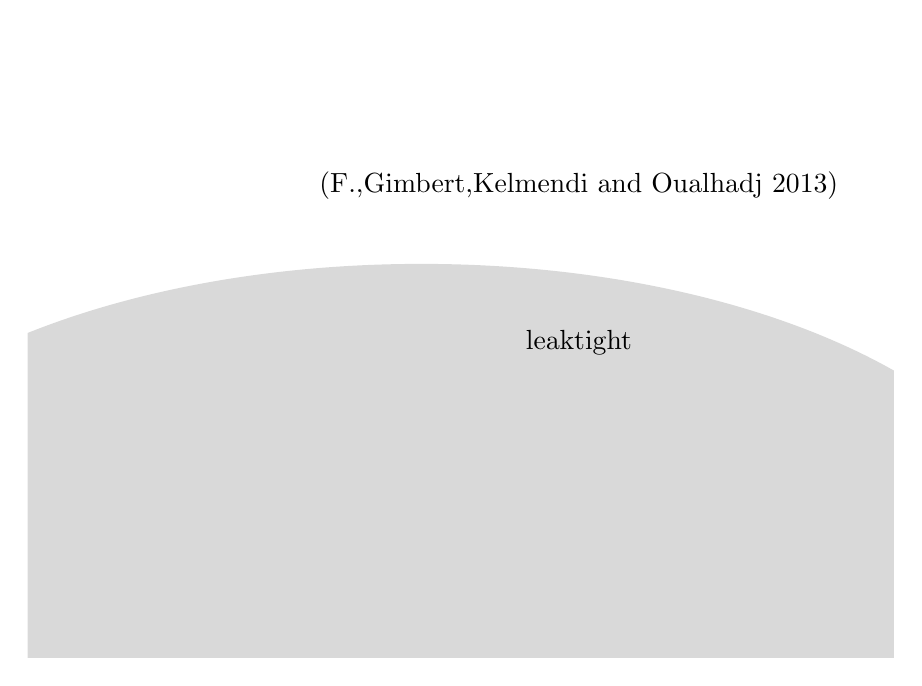
\begin{tikzpicture}
\clip (-6,0) rectangle (5,8);
\fill[white!85!black] (-1,1) ellipse (8cm and 4cm) ;
\draw (1,4) node {leaktight} ;
\draw (1,6) node {(F.,Gimbert,Kelmendi and Oualhadj 2013)} ;
\end{tikzpicture}
\end{frame}

\begin{frame}{Corollary}
\begin{center}
\begin{LARGE}
\textit{So far},\\
the Markov Monoid Algorithm is\\
the \textit{most correct} algorithm known\\

to solve the value $1$ problem. 
\pause

\vskip2em
But for \textit{how long}?
\end{LARGE}
\end{center}
\end{frame}

\subsection{On the optimality of the Markov Monoid Algorithm}

\begin{frame}{What it misses: different convergence speeds}

\begin{figure}
\begin{center}
\begin{picture}(60,35)(0,0)
	\gasset{Nw=7,Nh=7}

  	\node[Nmarks=i,iangle=-90](0)(30,15){$0$}
  	\node(L1)(0,10){$L_1$}
  	\node[Nmarks=r](L2)(0,30){$L_2$}
  	\node(R1)(60,10){$R_1$}
  	\node(R2)(60,30){$R_2$}

	\drawloop(0){$a$}

  	\drawedge[curvedepth=5,ELside=l](0,L1){$b,\frac{1}{2}$}
  	\drawedge[curvedepth=5,ELside=l](L1,0){$a,\frac{1}{4}$}
  	\drawedge(L1,L2){$b$}
	\drawloop[loopangle=-135](L1){$a,\frac{3}{4}$}
	\drawloop[loopangle=90](L2){$a,b$}

  	\drawedge[curvedepth=-5,ELside=r](0,R1){$b,\frac{1}{2}$}
  	\drawedge[curvedepth=-5,ELside=r](R1,0){$a,\frac{3}{4}$}
  	\drawedge[ELside=r](R1,R2){$b$}
	\drawloop[loopangle=-45](R1){$a,\frac{1}{4}$}
	\drawloop(R2){$a,b$}
\end{picture}
\end{center}
\end{figure}
$$\lim_n \prob{\AA}\left(b (a^n b)^{f(n)}\right) = 1\ \text{ if and only if }\ \lim_n f(n) \cdot \left(\frac{3}{4}\right)^n = \infty\ ,$$
\pause
\begin{center}
so $f(n) = 2^n$ works but $f(n) = n$ does not.
\end{center}
\end{frame}

\begin{frame}{A characterization}
$\ProProA$ is the space of prostochastic words.

$$A^*\ =\ \PPA{0}\ \subsetneq\ \PPA{1}\ \subsetneq\ \PPA{2}\ \subsetneq\ \cdots\ \subsetneq\ \ProProA\ .$$

\begin{lemma}
The following are equivalent:
\begin{itemize}
	\item The value $1$ problem over finite words,
	\item The emptiness problem over prostochastic words.
\end{itemize}
\end{lemma}

\pause
\begin{theorem}\hfill
\begin{enumerate}
	\item The Markov Monoid Algorithm answers ``YES'' if and only if
	there exists $x \in \PPA{1}$ accepted by $\AA$,
	\item The following problem is undecidable: determine whether
	there exists $x \in \PPA{2}$ accepted by $\AA$.
\end{enumerate}
\end{theorem}
\end{frame}

\begin{frame}{Prostochastic words}
\begin{definition}
$(u_n)_{n \in \NN}$ converges if for every $\AA$, the limit $\lim_n \P_\AA(u_n)$ exists.
\end{definition}
\pause
\begin{definition}
Two (converging) sequences $(u_n)_{n \in \NN}$ and $(v_n)_{n \in \NN}$ are equivalent if for every $\AA$,
$$\lim_n \P_\AA(u_n) > 0 \iff \lim_n \P_\AA(v_n) > 0\ .$$
\end{definition}
\pause
\begin{definition}
A prostochastic word is an equivalence class of converging sequences.
\end{definition}
\end{frame}

\begin{frame}{The $\omega$ operators}
\begin{definition}
Let $u$ be a converging sequence.

$u^{\omega_1}$ is the converging sequence $(u_n^{n!})_{n \in \NN}$.
\end{definition}
\pause
\begin{definition}
Let $u$ be a converging sequence.

$u^{\omega_k}$ is the converging sequence $(u_n^{(n!)^k})_{n \in \NN}$.
\end{definition}
\pause

\begin{example}
The prostochastic words $(a^{\omega_1} b)^{\omega_1}$ and $(a^{\omega_1} b)^{\omega_2}$ are not equal.
\end{example}
\end{frame}

\begin{frame}{An equivalent characterization}
\begin{theorem}
The Markov Monoid Algorithm answers ``YES'' if and only if
there exists a regular sequence $(u_n)_{n \in \NN}$ of finite words such that $\lim_n \prob{\AA}(u_n) = 1$.
\end{theorem}

The regular sequences are described by the following grammar:
$$u \quad = \quad a \quad \mid \quad u \cdot u \quad \mid \quad (u^n_n)_{n \in \NN}\ .$$
\end{frame}

%\begin{frame}{An equivalent characterization}
%\begin{theorem}
%The Markov Monoid Algorithm answers ``YES'' if and only if
%there exists $(u_n)_{n \in \NN}$ a sequence of finite words such that:
%\begin{enumerate}
%	\item $(u_n)_{n \in \NN}$ is of polynomial growth, \textit{i.e.} $|u_n| \le P(n)$ for some polynomial $P$,
%	\item $(\prob{\AA}(u_n))_{n \in \NN}$ converges exponentially fast to $1$, \textit{i.e.} 
%	$$\prob{\AA}(u_n) \ge 1 - P(n) \cdot C^{-n}\ ,$$
%	for some polynomial $P$ and constant $C > 1$.
%\end{enumerate}
%\end{theorem}
%\end{frame}

\begin{frame}{Corollary}
\begin{center}
\begin{LARGE}
In \textit{some} sense,
\vskip1em
the Markov Monoid Algorithm is\\
the \textit{most correct} algorithm\\
to solve the value $1$ problem. 
\end{LARGE}
\end{center}
\end{frame}

\section{Practice: ACM\'E}

\begin{frame}{ACM\'E}
\begin{verse}
The tool ACME (Automata with Counters, Monoids and Equivalence) has been written in OCaml by Nathana\"el Fijalkow and Denis Kuperberg.
\vskip1em

**********************************\\
Statistics on the Markov Monoid Algorithm:\\
**********************************\\
Automata that are leaktight and do not have value 1: 540\\
Automata that are leaktight and have value 1: 133\\
Automata that are not leaktight and may have value 1: 17\\
Automata that are not leaktight and have value 1: 310
\end{verse}
\end{frame}

\begin{frame}{The end.}
Thank you for your attention!
\end{frame}
\end{document}